!TEX root = main.tex
\renewcommand{\labelenumi}{\alph{enumi})}
\section*{Semanal 11}
\textbf{1. Diseña los PDA que acepten los siguientes lenguajes:}
\\
\begin{enumerate}
    \item Paréntesis balanceados y correctamente emparejados sobre el alfabeto $\Sigma$ = \{(,)\} y que acepte
    por estado de aceptación. \\
    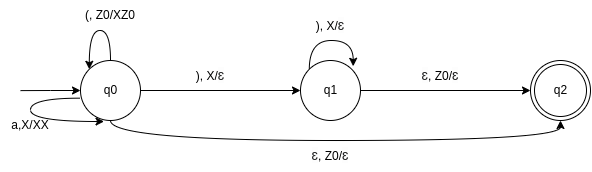
\includegraphics[scale=.70]{semanal11/1.png} \\
    \item $\{b^{n}a^{m} |$  m es el doble de n,n $>$ 0\} sobre el alfabeto $\Sigma$  = \{a,b\} y que acepte por pila vacía. \\
    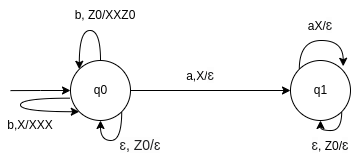
\includegraphics[scale=.70]{semanal11/2.png} \\
\end{enumerate}

\textbf{1. Transforma la aceptación de cada uno de los PDA anteriores al contrario, es decir, si acepta por
pila vacía, transfórmalo a que acepte por estado de aceptación, y viceversa.} \\


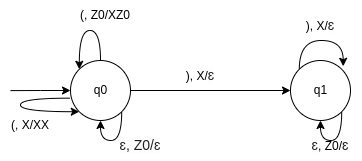
\includegraphics[scale=.70]{semanal11/3.png}

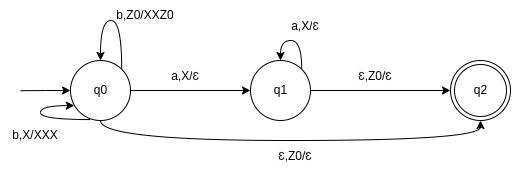
\includegraphics[scale=.70]{semanal11/4.png}




